\newpage
\section{ĐƯỜNG TIỆM CẬN CỦA ĐỒ THỊ HÀM SỐ}
\subsection{LÝ THUYẾT CẦN NHỚ}
%Trong phần này, ta giả thiết rằng hàm số $y=f(x)$ xác định trên $K$ ($K$ là khoảng, đoạn hoặc nửa khoảng).
\subsubsection{Tiệm cận ngang của đồ thị hàm số}
\indam\iconMT{Định nghĩa:}
	\begin{boxdn}
\immini{Đường thẳng $y=y_0$ gọi là \textbf{đường tiệm cận ngang} (gọi tắt là tiệm cận ngang) của đồ thị hàm số $y=f(x)$ nếu ít nhất một trong hai điều sau xảy ra
		\begin{itemize}
			\item $\lim\limits_{x\to+\infty}f(x)=y_0$
			\item $\lim\limits_{x\to-\infty}f(x)=y_0$
		\end{itemize}
		}{
	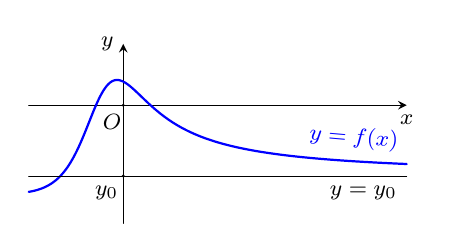
\begin{tikzpicture}[>=stealth,line join=round,line cap=round,font=\footnotesize,scale=.6]
			\def\a{-1.5} \def\b{0} \def\c{0.5} \def\m{1} \def\n{1}  \def\p{1}
%			\clip (-4,-4) rectangle (4,2);
			\draw[->] (-2,0)--(6,0)node[below]{$x$};
			\draw[->] (0,-2.5)--(0,1.3)node[left]{$y$};
			\fill (0,0)circle(1pt)node[xshift=-4,yshift=-6]{$O$};
			\fill (0,-1.5)circle(1pt)node[xshift=-6,yshift=-6]{$y_0$};
			\draw[thick,blue,samples=200,smooth,domain=-2:6] plot(\x,{(\a*(\x)^2+\b*\x+\c)/(\m*(\x)^2+\n*\x+\p)}) node[above left, rotate=-5]{$y=f(x)$};
			\draw[samples=200,smooth,domain=-2:6] plot(\x,{\a/\m})node [below left]{$y=y_0$};	
	\end{tikzpicture}
}
	\end{boxdn}	
\begin{khung4}{Ghi nhớ 1}		
		$\bullet$ Tiệm cận ngang của đồ thị hàm số là hình ảnh hình học của \textbf{giới hạn tại vô cực} của hàm số đó.\\
		$\bullet$ Đồ thị hàm số đa thức không có tiệm cận ngang.\\
		$\bullet$ Tập xác định của hàm số không chứa khoảng vô cực thì đồ thị không có đường tiện cận ngang.		
\end{khung4}
\subsubsection{Tiệm cận đứng của đồ thị hàm số}
\indam\iconMT{Định nghĩa:}
\begin{boxdn}
\immini{Đường thẳng $x=x_0$ gọi là \textbf{đường tiệm cận đứng} (gọi tắt là tiệm cận đứng) của đồ thị hàm số $y=f(x)$ nếu ít nhất một trong bốn điều sau xảy ra
\begin{multicols}{2}
	\begin{itemize}
	\item $\lim\limits_{x\to x_0^+} f(x)=+\infty$
	\item $\lim\limits_{x\to x_0^-} f(x)=-\infty$
	\item $\lim\limits_{x\to x_0^+}f(x)=-\infty$
	\item $\lim\limits_{x\to x_0^-} f(x)=+\infty$
	\end{itemize}
\end{multicols}
	}{
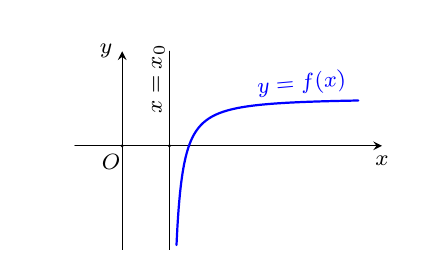
\begin{tikzpicture}[>=stealth,line join=round,line cap=round,font=\footnotesize,scale=.6]
	\def\a{1} \def\b{0} \def\c{-2} \def\m{1} \def\n{0}  \def\p{-1}
	\clip (-2,-2.2) rectangle (6,2.5);
	\draw[->] (-1,0)--(5.5,0)node[below]{$x$};
	\draw[->] (0,-2.2)--(0,2)node[left]{$y$};
	\fill (0,0)circle(1pt)node[xshift=-4,yshift=-6]{$O$}
	(1,0) circle(1pt);
	\draw[thick,blue,samples=200,smooth,domain=1.15:5] plot(\x,{(\a*(\x)^2+\b*\x+\c)/(\m*(\x)^2+\n*\x+\p)}) node[above left, rotate=5]{$y=f(x)$};
	\draw (1,-2.2)--(1,2) node[xshift=-4,yshift=-10, rotate=90]{$x=x_0$};
\end{tikzpicture}	
}
\end{boxdn}	
\begin{khung4}{Ghi nhớ 2}		
	$\bullet$ Tiệm cận đứng của đồ thị hàm số là hình ảnh hình học của \textbf{giới hạn vô cực} của hàm số đó.\\
	$\bullet$ Đồ thị hàm số có tập xác định $\mathbb{R}$ không có tiệm cận đứng.
\end{khung4}
\subsubsection{Tiệm cận xiên của đồ thị hàm số}
\indam\iconMT{Định nghĩa:}
\begin{boxdn}
\immini{Đường thẳng $y=ax+b$ ($a\neq0$) gọi là \textbf{đường tiệm cận xiên} (gọi tắt là tiệm cận xiên) của đồ thị hàm số $y=f(x)$ nếu ít nhất một trong hai điều sau xảy ra 
		\begin{itemize}
			\item $\lim\limits_{x\to+\infty}\left[f(x)-(ax+b)\right]=0$
			\item $\lim\limits_{x\to-\infty}\left[f(x)-(ax+b)\right]=0$
		\end{itemize}
}{
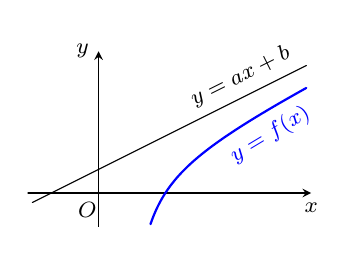
\begin{tikzpicture}[>=stealth,line join=round,line cap=round,font=\footnotesize,scale=.6]
	\def\a{1} \def\b{0} \def\c{-2} \def\m{0} \def\n{2}  \def\p{-1}
	\clip (-1.5,-0.7) rectangle (5,3.5);
	\draw[->] (-1.5,0)--(4.5,0)node[below]{$x$};
	\draw[->] (0,-1.5)--(0,3)node[left]{$y$};
	\fill (0,0)circle(1pt)node[xshift=-4,yshift=-6]{$O$};
	\draw[thick,blue,samples=200,smooth,domain=1.1:4.4] plot(\x,{(\a*(\x)^2+\b*\x+\c)/(\m*(\x)^2+\n*\x+\p)}) node[below left, rotate=31]{$y=f(x)$};
	\draw[samples=200,smooth,domain=-1.4:4.4] plot(\x,{\a/\n*\x+\b-(\a*\p/\n)})node [above left, rotate=26.5]{$y=ax+b$};	
	\end{tikzpicture}	
}
\end{boxdn}	
\begin{khung4}{Ghi nhớ 3}		
		$\bullet$ Đường thẳng $y=ax+b$ ($a\neq0$) là tiệm cận xiên của đồ thị hàm số $y=f(x)$ khi và chỉ khi 
\[a=\lim\limits_{x\to+\infty}\dfrac{f(x)}{x}{\ }\text{và}{\ }b=\lim_{x\to+\infty}[f(x)-ax] {\ } \text{hoặc}{\ } a=\lim\limits_{x\to-\infty}\dfrac{f(x)}{x}{\ }\text{và}{\ }b=\lim_{x\to-\infty}[f(x)-ax].\]
		$\bullet$ Nếu $f(x)=mx+n+\dfrac{r}{px+q}$, trong đó $mpr\neq0$ thì đường thẳng $y=mx+n$ là tiệm cận xiên của đồ thị hàm số.
\end{khung4}

%-------------------------------------------------------------------------------------------------------------
\subsection{PHÂN LOẠI VÀ PHƯƠNG PHÁP GIẢI TOÁN}
%%%Dang1%
\begin{dang}{Xác định các đường tiệm cận của đồ thị hàm số cho bởi bảng biến thiên hoặc đồ thị}
	\begin{listEX}[1]
		\item [\ding{172}] Xác định các giới hạn vô cực và tại vô cực (nếu có) của hàm số $y=f(x)$.
		\item [\ding{173}] Nếu $\lim\limits_{x\to x_0^+}f(x)=+\infty$ hoặc $\lim\limits_{x\to x_0^-}f(x)=+\infty$ hoặc $\lim\limits_{x\to x_0^+}f(x)=-\infty$ hoặc $\lim\limits_{x\to x_0^-}f(x)=-\infty$ thì đồ thị hàm số có \textbf{đường tiệm cận đứng} là $x=x_0$.\\
		Nếu $\lim\limits_{x\to+\infty}f(x)=y_0$ hoặc $\lim\limits_{x\to-\infty}f(x)=y_0$ thì đồ thị hàm số có \textbf{đường tiệm cận ngang} là $y=y_0$.\\
		Nếu $\begin{cases}\lim\limits_{x\to+\infty}\dfrac{f(x)}{x}=a \\ \lim\limits_{x\to+\infty}\left[f(x)-ax\right]=b
		\end{cases}$
		 hoặc 
		 $\begin{cases}\lim\limits_{x\to-\infty}\dfrac{f(x)}{x}=a \\ \lim\limits_{x\to-\infty}\left[f(x)-ax\right]=b
\end{cases}$
		 thì đồ thị hàm số có \textbf{đường tiệm cận xiên} là $y=ax+b$.
	\end{listEX}
	\end{dang}	
%%%Vidu1.1%
\begin{vd}%[2D1N4-1]%[Dự án đề cương 3 Khối NH24-25-Dot 1- Bùi Lương Phúc]
Giả sử hàm số $y=f(x)$ có bảng biến thiên như sau:
\begin{center}

\begin{tikzpicture}
	\tkzTabInit[nocadre=true, lgt=1, espcl=4, deltacl=0.5]
	{$x$/0.7,$y’$/0.7,$y$/1.5}
	{$0$,$2$,$+\infty$}
	\tkzTabLine{,+,d,+,}
	\tkzTabVar{-/$-10$,+D-/$+\infty$/$-\infty$,
		+/$10$}
\end{tikzpicture}
\end{center}
Hãy tìm các đường tiệm cận đứng và tiệm cận ngang của đồ thị hàm số đã cho.
	\loigiai{Từ bảng biến thiên ta có
\begin{itemize}
	\item $\lim\limits_{x\to2^-}f(x)=+\infty$. Suy ra đường thẳng $x=2$ là một tiệm cận đứng của đồ thị hàm số. 
	\item $\lim\limits_{x\to2^+}f(x)=-\infty$. Suy ra đường thẳng $x=2$ là một tiệm cận đứng của đồ thị hàm số. 
	\item $\lim\limits_{x\to+\infty}f(x)=10$. Suy ra đường thẳng $y=10$ là một tiệm cận ngang của đồ thị hàm số.\\
Vậy đồ thị hàm số đã cho có $1$ tiệm cận đứng là đường thẳng $x=2$ và $1$ tiệm cận ngang là đường thẳng $y=10$.	
\end{itemize}
}
\end{vd}
%%%Vidu1.2%
\begin{vd}%[2D1H4-1]%[Dự án đề cương 3 Khối NH24-25-Dot 1- Bùi Lương Phúc]
\immini{Cho hàm số $y=\dfrac{ax^2+bx+c}{mx+n}$ có đồ thị như hình bên.\\
	Hãy tìm các đường tiệm cận đứng và tiệm cận xiên của đồ thị hàm số đã cho.}{
	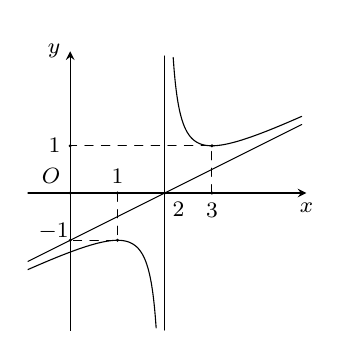
\begin{tikzpicture}[>=stealth,line join=round,line cap=round,font=\footnotesize,scale=.6]
		\def\a{0.5} \def\b{-1} \def\c{1} \def\d{-2}
		\clip (-0.9,-2.9) rectangle (5.5,3.5);
		\draw[->] (-1,0)--(5,0)node[below]{$x$};
		\draw[->] (0,-3)--(0,3)node[left]{$y$};
		\fill (0,0)circle(1pt)node[above left]{$O$};
		\fill (0,-1)circle(1pt)node[xshift=-6,yshift=3]{$-1$};
		\fill (1,0)circle(1pt)node[above]{$1$};
		\fill (3,0)circle(1pt)node[below]{$3$};
		\fill (0,1)circle(1pt)node[left]{$1$};
		\fill (2,0)circle(1pt)node[xshift=5,yshift=-6]{$2$};
		\fill (3,1)circle(1pt) (1,-1)circle(1pt);
		\draw (2,-2.9)--(2,2.9);
		\draw[dashed](1,0)|-(0,-1) (3,0)|-(0,1);
		\draw[samples=150,smooth,domain=-0.9:1.82] plot(\x,{\a*\x+\b+0.5/(\c*\x+\d)});
		\draw[samples=150,smooth,domain=2.18:4.9] plot(\x,{\a*\x+\b+0.5/(\c*\x+\d)});
		\draw[samples=150,smooth,domain=-0.9:4.9] plot(\x,{\a*\x+\b});
		\end{tikzpicture}}
	\loigiai{Từ hình vẽ ta có
		\begin{itemize}
			\item Đồ thị hàm số nhận đường thẳng $x=2$ là một tiệm cận đứng. 
			\item Đồ thị hàm số nhận đường thẳng $d\colon y=ax+b$ là một tiệm cận xiên, trong đó $d$ đi qua hai điểm $(0;-1)$ và $(2;0)$.
			Ta có 
			$\begin{cases}a\cdot0+b=-1 \\a\cdot2+b=0\end{cases}
			\Leftrightarrow\begin{cases}b=-1 \\a=\dfrac{1}{2}.\end{cases}$.\\
			Vậy đồ thị hàm số đã cho có $1$ tiệm cận đứng là đường thẳng $x=1$ và $1$ tiệm cận xiên là đường thẳng $y=\dfrac{1}{2}x-1$.	
		\end{itemize}
	}
\end{vd}
%%%Dang2%
\begin{dang}{Tìm đường tiệm cận của đồ thị hàm số cho bởi công thức}
	\begin{listEX}[1]
		\item [\ding{172}] Tìm tập xác định của hàm số $y=f(x)$. 
		\item [\ding{173}] Tính các giới hạn vô cực và tại vô cực (nếu có).
		\item [\ding{174}] Giả sử hàm số có tập xác định là $\mathscr{D}=\mathbb{R}\setminus \{x_0\}$. \\
		Nếu $\lim\limits_{x\to+\infty}f(x)=y_0$ hoặc $\lim\limits_{x\to-\infty}f(x)=y_0$ thì đồ thị hàm số có \textbf{đường tiệm cận ngang} là $y=y_0$.\\
		Nếu $\lim\limits_{x\to x_0^+}f(x)=+\infty$ hoặc $\lim\limits_{x\to x_0^-}f(x)=+\infty$ hoặc $\lim\limits_{x\to x_0^+}f(x)=-\infty$ hoặc $\lim\limits_{x\to x_0^-}f(x)=-\infty$ thì đồ thị hàm số có \textbf{đường tiệm cận đứng} là $x=x_0$.\\
		Nếu $\lim\limits_{x\to+\infty}[f(x)-(ax+b)]=0$ hoặc $\lim\limits_{x\to-\infty}[f(x)-(ax+b)]=0$ (với $a\neq0$) thì đồ thị hàm số có \textbf{đường tiệm cận xiên} là $y=ax+b$.
	\end{listEX}
		\textbf{LƯU Ý}\\
	$\bullet$ Đối với hàm số $y=\dfrac{ax+b}{cx+d}$, ($c\neq0$,$ad-bc\neq0$), đồ thị có $1$ tiệm đứng là $x=-\dfrac{d}{c}$ và $1$ tiệm cận ngang $y=\dfrac{a}{c}$.\\
	$\bullet$ Đối với hàm số $y=mx+n+\dfrac{r}{px+q}$, ($mpr\neq0$), đồ thị có $1$ tiệm đứng là $x=-\dfrac{q}{p}$ và $1$ tiệm cận xiên $y=mx+n$.		
\end{dang}
%%%Vidu2.1%
\begin{vd}%[2D1N4-1]%[Dự án đề cương 3 Khối NH24-25-Dot 1- Bùi Lương Phúc]
		(\textit{\footnotesize Trích đề thi CKI - THPT Số 1 Văn Bàn - Năm học 2024-2025})\\
	Đường tiệm cận ngang của đồ thị hàm số $y=\dfrac{2\,024x+2\,025}{x-5}$ là
	\choice
	{$y=2\,025$}
	{\True $y=2\,024$}
	{$y=1$}
	{$y=-5$}
	\loigiai{
	Hàm số đã cho có tập xác định là $\mathbb{R} \setminus \{5\}$. \\
		Ta có $\lim\limits_{x \to \pm\infty} \dfrac{2\,024x+2\,025}{x-5}=
		\lim\limits_{x \to \pm\infty} \dfrac{2\,024 + \dfrac{2\,025}{x}}{1 - \dfrac{5}{x}}=2\,024$.\\
		Vậy đường tiệm cận ngang của đồ thị hàm số là $y = 2\,024$.
	}
\end{vd}
%%%Vidu2.2%
\begin{vd}%[2D1H4-1]%[Dự án đề cương 3 Khối NH24-25-Dot 1- Bùi Lương Phúc]
Tìm các đường tiệm cận của đồ thị mỗi hàm số sau:
\begin{multicols}{2}
\begin{itemize}
\item[a)] $y = \dfrac{x}{2 - x}$;
\item[b)] $y =\dfrac{x^2+2x+3}{x}$.
\end{itemize}
\end{multicols}
\loigiai{
\begin{itemize}
\item[a)] Hàm số đã cho có tập xác định là $\mathbb{R} \setminus \{2\}$. \\
Ta có
\[\lim_{x \to +\infty} y = \lim_{x \to +\infty} \dfrac{x}{2 - x} = -1; \quad
\lim_{x \to -\infty} y = \lim_{x \to -\infty} \dfrac{x}{2 - x} = -1.
\]
Suy ra đường thẳng $y = -1$ là tiệm cận ngang của đồ thị hàm số đã cho.\\
Ta có
\[\lim_{x \to 2^-} y = \lim_{x \to 2^-} \dfrac{x}{2 - x} = +\infty
;\qquad \lim_{x \to 2^+} y = \lim_{x \to 2^+} \dfrac{x}{2 - x} = -\infty.
\]
Suy ra đường thẳng $x = 2$ là tiệm cận đứng của đồ thị hàm số đã cho.\\
Tóm lại, đồ thị hàm số đã cho có hai đường tiệm cận là $y = -1$ và $x = 2$.
\item[b)] Hàm số đã cho có tập xác định là $\mathbb{R} \setminus \{0\}$. \\
Viết lại $y = \dfrac{x^2+2x+3}{x}=x +2 + \dfrac{3}{x}$.\\
Ta có
\[\lim_{x \to 0^-} y = \lim_{x \to 0^-} \left(x +2 + \dfrac{3}{x}\right) = -\infty; \quad
\lim_{x \to 0^+} y = \lim_{x \to 0^+} \left(x +2 + \dfrac{3}{x}\right)  = +\infty.
\]
Suy ra đường thẳng $x = 0$ là tiệm cận đứng của đồ thị hàm số đã cho.\\
Ta có
\[\lim_{x \to -\infty} \left[y-(x+2)\right] = \lim_{x \to -\infty} \dfrac{3}{x} = 0; \quad
\lim_{x \to +\infty} \left[y-(x+2)\right] = \lim_{x \to +\infty} \dfrac{3}{x} = 0.
\]
Suy ra đường thẳng $y = x +2$ là tiệm cận xiên của đồ thị hàm số đã cho.\\
Tóm lại, đồ thị hàm số đã cho có hai đường tiệm cận là $x = 0$ và $y=x+2$.
\end{itemize}
}
\end{vd}
%%%Vidu2.3%
\begin{vd}%[2D1V4-1]%[Dự án đề cương 3 Khối NH24-25-Dot 1- Bùi Lương Phúc]
Tìm các đường tiệm cận của đồ thị hàm số $y = \dfrac{2x+1}{\sqrt{x^2-1}}$.
\loigiai{
Hàm số đã cho có tập xác định là $\mathscr{D}=(-\infty;-1)\cup(1;+\infty)$. \\
Ta có\\
$\bullet\ \lim\limits_{x \to {-1}^-} y = \lim\limits_{x \to {-1}^-} \dfrac{2x+1}{\sqrt{x^2-1}}= -\infty$. Suy ra đồ thị hàm số có tiệm cận đứng $x=-1$.\\
$\bullet\ \lim\limits_{x \to 1^+} y = \lim\limits_{x \to 1^+} \dfrac{2x+1}{\sqrt{x^2-1}}= +\infty$. Suy ra đồ thị hàm số có tiệm cận đứng $x=1$.\\
$\bullet\ \lim\limits_{x \to -\infty} y = \lim\limits_{x \to -\infty} \dfrac{2x+1}{\sqrt{x^2-1}}=\lim\limits_{x \to -\infty} \dfrac{2+\dfrac{1}{x}}{-\sqrt{1-\dfrac{1}{x^2}}}= -2$. Suy ra đồ thị hàm số có tiệm cận ngang $y=-2$.\\
$\bullet\ \lim\limits_{x \to +\infty} y = \lim\limits_{x \to +\infty} \dfrac{2x+1}{\sqrt{x^2-1}}= \lim\limits_{x \to +\infty} \dfrac{2+\dfrac{1}{x}}{\sqrt{1-\dfrac{1}{x^2}}}=2$. Suy ra đồ thị hàm số có tiệm cận ngang $y=2$.\\
Tóm lại, đồ thị hàm số đã cho có bốn đường tiệm cận là $x = -1$, $x = 1$, $y = -2$ và $y=2$.
}
\end{vd}
%%%Dang3%
\begin{dang}{Bài toán thực tế và ý nghĩa của tiệm cận}
	\begin{listEX}[1]
		\item [\ding{172}] Nếu $f(t)$ đồng biến trên khoảng $(0;+\infty)$ và $\lim\limits_{t\to+\infty}f(t)=T$ thì ta bảo rằng: Khi $t$ đủ lớn (rất lớn), $f(t)$ tiến dần đến mức $T$ ($T$ là ngưỡng trên).
		\item [\ding{173}] Nếu $f(t)$ nghịch biến trên khoảng $(0;+\infty)$ và $\lim\limits_{t\to+\infty}f(t)=T$ thì ta bảo rằng: Khi $t$ đủ lớn (rất lớn), $f(t)$ giảm dần về mức $T$ ($T$ là ngưỡng dưới).
	\end{listEX}
\end{dang}
%%%Vidu3%
\begin{vd}%[2D1V4-4]%[Dự án đề cương 3 Khối NH24-25-Dot 1- Bùi Lương Phúc]
Số lượng sản phẩm bán được của một công ty trong $x$\,tháng được tính theo công thức
$S(x) = 200 \left( \dfrac{5x}{2 + x} \right)$,\ trong đó $x > 1$ (\textit{Nguồn: R. Larson and B. Edwards, Calculus 10e, Cengage 2014}).
\begin{itemize}
\item[a)] Xem $y = S(x)$ là một hàm số xác định trên nửa khoảng $[1; +\infty)$, tìm tiệm cận ngang của đồ thị hàm số đó.
\item[b)] Nêu nhận xét về số lượng sản phẩm bán được của công ty đó trong $x$\,tháng khi $x$ rất lớn.
\end{itemize}
\loigiai{
\begin{itemize}
\item[a)]
Ta có $\lim\limits_{x \to +\infty} S(x) = \lim\limits_{x \to +\infty} 200 \left( \dfrac{5x}{2 + x} \right) = 200 \cdot \lim\limits_{x \to +\infty} \dfrac{5x}{2 + x} = 200 \cdot 5 = 1000$.\\
Vậy đường thẳng $y = 1\,000$ là tiệm cận ngang của đồ thị hàm số $y = S(x)$.
\item[b)] Ta có đồ thị hàm số $y=S(x)$ nhận đường thẳng $y = 1000$ làm tiệm cận ngang, tức là khi $x$ đủ lớn thì số lượng sản phẩm bán được của công ty đó trong $x$ (tháng) sẽ tiến gần đến mức $1\,000$ và số lượng sản phẩm bán không thể vượt mức $1\,000$ cho dù thời gian $x$ có kéo dài đến vô cùng.
\end{itemize}
}
\end{vd}

%-----------------------------------------------------------------------------
\subsection{Bài tập rèn luyện}
\ind{PHẦN I.} \inden{Câu trắc nghiệm nhiều phương án lựa chọn. Mỗi câu hỏi học sinh chỉ chọn một phương án.}\\
\setcounter{ex}{0}
\Opensolutionfile{ans}[ans/2D1-Bai3-TN]%--Đặt tên 2D1-Bai3-Dang1-TN
%%%Câu 1%
\begin{ex}%[2D1-Bai3-Dang1-TN]%[Dự án đề cương 3 Khối NH24-25-Dot 1- Bùi Lương Phúc]%[2D1N4-1]
	(\textit{\footnotesize Trích đề thi GKI - THPT Phạm Văn Đồng - Năm học 2024-2025})\\
	Tiệm cận ngang của đồ thị hàm số $y=\dfrac{5x-10}{x+10}$ là đường thẳng có phương trình
	\choice
	{\True $ y=5$}
	{$ y=0$}
	{$ y=-10$}
	{$ y=-1$}
	\loigiai{
		Hàm số đã cho có tập xác định là $\mathbb{R} \setminus \{-10\}$. \\
		Vì $\underset{x\to\pm\infty}{\lim}\,y=\underset{x\to\pm\infty}{\lim}\,\dfrac{5x-10}{x+10}=\underset{x\to\pm\infty}{\lim}\,\dfrac{5-\dfrac{10}{x}}{1+\dfrac{10}{x}}=5$ nên đường thẳng $ y=5$ là đường tiệm cận ngang của đồ thị hàm số.
		}
\end{ex}
%%%Câu 2%
\begin{ex}%[2D1-Bai3-Dang1-TN]%[Dự án đề cương 3 Khối NH24-25-Dot 1- Bùi Lương Phúc]%[2D1N4-1]
	(\textit{\footnotesize Trích đề thi CKI - THPT Thực Hành Sư Phạm - Năm học 2024-2025})\\
	Tiệm cận ngang của đồ thị hàm số $y=\dfrac{1+4x}{x-1}$ là
	\choice
	{$y=1$}
	{\True $y=4$}
	{$y=-1$}
	{$y=-4$}
	\loigiai{
		Hàm số đã cho có tập xác định là $\mathbb{R} \setminus \{1\}$. \\
		Ta có $\lim\limits_{x\to+\infty}\dfrac{1+4x}{x-1}=4$ và $\lim\limits_{x\to-\infty}\dfrac{1+4x}{x-1}=4$  nên đồ thị hàm số có 1 đường tiệm cận ngang là $y=4$.
	}
\end{ex}
%%%Câu 3%
\begin{ex}%[2D1-Bai3-Dang1-TN]%[Dự án đề cương 3 Khối NH24-25-Dot 1- Bùi Lương Phúc]%[2D1N4-1]
	(\textit{\footnotesize Trích đề thi CKI - DTNT Tỉnh Phú Yên - Năm học 2024-2025})\\
	Tiệm cận đứng của đồ thị hàm số $y=\dfrac{4x^2-x+1}{3x+2}$ là đường thẳng
	\choice
	{\True $x=-\dfrac{2}{3}$}
	{$x=\dfrac{2}{3}$}
	{$x=\dfrac{4}{3}$}
	{$x=-\dfrac{3}{2}$}
	\loigiai{Tiệm cận đứng của đồ thị hàm số $y=\dfrac{4x^2-x+1}{3x+2}$ là $x=-\dfrac{2}{3}$.}
\end{ex}
%%%Câu 4%	
\begin{ex}%[2D1-Bai3-Dang1-TN]%[Dự án đề cương 3 Khối NH24-25-Dot 1- Bùi Lương Phúc]%[2D1N4-1]
	(\textit{\footnotesize Trích đề thi CKI - THPT Nguyễn Thái Bình - Năm học 2024-2025})\\
	Đường tiệm cận ngang của đồ thị hàm số $y=\dfrac{3x-1}{x+2}$ có phương trình là
	\choice
	{$y=-\dfrac{1}{2}$}
	{\True $y=3$}
	{$x=3$}
	{$x=-2$}
	\loigiai{
		Hàm số đã cho có tập xác định là $\mathbb{R} \setminus \{-2\}$. \\
		Đường tiệm cận ngang của đồ thị hàm số $y=\dfrac{3x-1}{x+2}$ có phương trình $y=3$.
	}
\end{ex}	
%%%Câu 5%
\begin{ex}%[2D1-Bai3-Dang1-TN]%[Dự án đề cương 3 Khối NH24-25-Dot 1- Bùi Lương Phúc]%[2D1N4-1]
Tiệm cận đứng của đồ thị hàm số $y = \dfrac{3x + 1}{x - 2}$ là đường thẳng
\choice
{\True $x = 2$ }
{$x = \dfrac{1}{3}$ }
{$y = 3$ }
{$y = \dfrac{1}{3}$}
\loigiai{
Hàm số đã cho có tập xác định là $\mathbb{R} \setminus \{2\}$. \\
Vì $\lim\limits_{x\to2^+}y=+\infty$, $\lim\limits_{x\to2^-}y=-\infty$ nên đường thẳng $x=2$ là một tiệm cận đứng của đồ thị hàm số.
}
\end{ex}
%%%Câu 6%
\begin{ex}%[2D1-Bai3-Dang1-TN]%[Dự án đề cương 3 Khối NH24-25-Dot 1- Bùi Lương Phúc]%[2D1H4-1]
Tiệm cận ngang của đồ thị hàm số $y = \dfrac{5x - 3}{x + 5}$ là đường thẳng đi qua điểm nào sau đây?
\choice
{$M(-5;0)$ }
{$N\left(\dfrac{3}{5};0\right)$ }
{\True $P(1;5)$ }
{$Q(5;0)$}
\loigiai{
Hàm số đã cho có tập xác định là $\mathbb{R} \setminus \{-5\}$. \\
Vì $\lim\limits_{x\to\pm\infty}y=5$ nên đường thẳng $y=5$ là một tiệm cận ngang của đồ thị hàm số.\\
Đường thẳng $y=5$ đi qua điểm $P(1;5)$.
}
\end{ex}
%%%Câu 7%
\begin{ex}%[2D1-Bai3-Dang1-TN]%[Dự án đề cương 3 Khối NH24-25-Dot 1- Bùi Lương Phúc]%[2D1N4-1]
Tiệm cận xiên của đồ thị hàm số $y = 2x - \dfrac{1}{x + 1}$ là đường thẳng
\choice
{\True $y = 2x$ }
{$y = x + 1$ }
{$y = 2x - 1$ }
{$y = 2x + 1$}
\loigiai{
Hàm số đã cho có tập xác định là $\mathbb{R} \setminus \{-1\}$. \\
Vì $\lim\limits_{x \to \pm\infty} (y-2x)= \lim\limits_{x \to \pm\infty} \dfrac{-1}{x+1} = 0$ nên đường thẳng $y = 2x$ là tiệm cận xiên của đồ thị hàm số đã cho.
}
\end{ex}
%%%Câu 8%
\begin{ex}%[2D1-Bai3-Dang2-TN]%[Dự án đề cương 3 Khối NH24-25-Dot 1- Bùi Lương Phúc]%[2D1N4-1]
	(\textit{\footnotesize Trích đề thi CKI - THPT Phan Ngọc Hiền - Năm học 2024-2025})\\
	\immini{Cho hàm số $y=\dfrac{ax+b}{cx+d}$, ($c \neq 0$, $ad-bc \neq 0$) có đồ thị là đường cong trong hình bên. Tiệm cận ngang của đồ thị hàm số đã cho có phương trình là
		\choice[2]
		{$x=-1$}
		{$y=-1$}
		{\True $y=1$}
		{$x=1$}}
	{\begin{tikzpicture}[scale=0.5,>=stealth, font=\footnotesize, line join=round, line cap=round]
			\def\a{1} \def\b{1} \def\c{1} \def\d{-1}
			\def\xmin{-3} \def\xmax{5}
			\def\ymin{-3} \def\ymax{5}
			\draw[->] (\xmin,0)--(\xmax,0) node [below]{$x$};
			\draw[->] (0,\ymin)--(0,\ymax) node [left]{$y$};
			\node at (0,0) [above left]{$O$};
			\clip (\xmin+0.1,\ymin+0.1) rectangle (\xmax-0.1,\ymax-0.1);
			\draw[smooth,samples=200,domain=\xmin:(-\d/\c-0.1)] plot(\x,{(\a*(\x)+\b)/(\c*(\x)+\d)});
			\draw[smooth,samples=200,domain=(-\d/\c+0.1:\xmax)] plot(\x,{(\a*(\x)+\b)/(\c*(\x)+\d)});
			\draw (-\d/\c,\ymin)--(-\d/\c,\ymax) (\xmin,\a/\c)--(\xmax,\a/\c);
			\draw (1,0) node[below right]{$1$}circle(1pt);
			\draw (0,1) node[above right]{$1$}circle(1pt);
			\draw (-1,0) node[below]{$-1$}circle(1pt);
			\draw (0,-1) node[left]{$-1$}circle(1pt);	
			\draw (1,1) circle(1pt);															
	\end{tikzpicture}}
	\loigiai{
		Tiệm cận ngang của đồ thị hàm số đã cho có phương trình là $y=1$.
	}
\end{ex}
%%%Câu 9%
\begin{ex}%[2D1-Bai3-Dang2-TN]%[Dự án đề cương 3 Khối NH24-25-Dot 1- Bùi Lương Phúc]%[2D1H4-1]
\immini{Cho hàm số $y = f(x)$ xác định trên $\mathbb{R} \setminus \{1\}$ và có đồ thị như hình bên. Phương trình các đường tiệm cận đứng và tiệm cận xiên của đồ thị hàm số là
\choice [2]
{\True $x = 1$ và $y = -x$}
{$x = 1$ và $y = -x$}
{$x = 1$ và $y = 2x$}
{$x = -1$ và $y = -x$}
}{
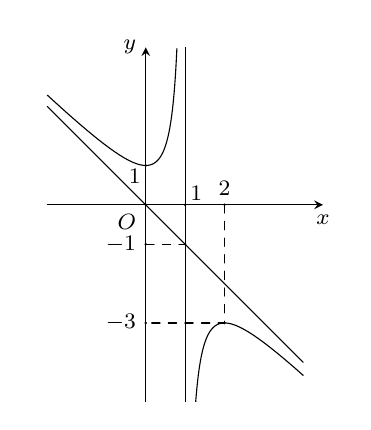
\begin{tikzpicture}[>=stealth,line join=round,line cap=round,font=\footnotesize,scale=.5]
\def\a{-1} \def\b{0} \def\c{1} \def\d{-1}
\clip (-3,-5) rectangle (5,4.5);
\draw[->] (-2.5,0)--(4.5,0)node[below]{$x$};
\draw[->] (0,-5)--(0,4)node[left]{$y$};
\fill (0,0)circle(1pt)node[below left]{$O$};
\fill (0,1)circle(1pt)node[yshift=-4,xshift=-4]{$1$};
\fill (0,-1)circle(1pt)node[left]{$-1$};
\fill (0,-3)circle(1pt)node[left]{$-3$};
\fill (1,0)circle(1pt)node[xshift=4,yshift=4]{$1$};
\fill (2,0)circle(1pt)node[above]{$2$};
\fill (2,-3)circle(1pt) (1,-1)circle(1pt) ;
\draw (1,-5)--(1,4);
\draw[dashed](2,0)|-(0,-3) (0,-1)--(1,-1);
\draw[samples=150,smooth,domain=-2.5:0.79] plot(\x,{\a*\x+\b-1/(\c*\x+\d)});
\draw[samples=150,smooth,domain=1.24:4] plot(\x,{\a*\x+\b-1/(\c*\x+\d)});
\draw[samples=150,smooth,domain=-2.5:4] plot(\x,{\a*\x+\b});
\end{tikzpicture}
}
\loigiai{Từ hình vẽ ta có
\begin{itemize}
\item Đồ thị hàm số nhận đường thẳng $x=1$ là một tiệm cận đứng.
\item Đồ thị hàm số nhận đường thẳng $d\colon y=ax+b$ là một tiệm cận xiên, trong đó $d$ đi qua hai điểm $(0;0)$ và $(1;-1)$.
Ta có
$\begin{cases}a\cdot0+b=0 \\a\cdot1+b=-1\end{cases}
\Leftrightarrow\begin{cases}b=0 \\a=-1.\end{cases}$.\\
Vậy đồ thị hàm số đã cho có $1$ tiệm cận đứng là đường thẳng $x=1$ và $1$ tiệm cận xiên là đường thẳng $y=-x$.
\end{itemize}
}
\end{ex}
%%%Câu 10%
\begin{ex}%[2D1-Bai3-Dang1-TN]%[Dự án đề cương 3 Khối NH24-25-Dot 1- Bùi Lương Phúc]%[2D1H4-1]
Giao điểm $I$ của hai đường tiệm cận của đồ thị hàm số $y = \dfrac{-5x + 3}{x + 1}$ là
\choice
{\True $I(-1; -5)$ }
{$I(0; -5)$ }
{$I(0; 5)$ }
{$I(1; -5)$	}
\loigiai{
Hàm số đã cho có tập xác định là $\mathbb{R} \setminus \{-1\}$. \\
Vì $\lim\limits_{x\to-1^-}y=-\infty$, $\lim\limits_{x\to-1^+}y=+\infty$ nên đồ thị hàm số có tiệm cận đứng là đường thẳng $x = -1$.\\
Vì $\lim\limits_{x\to\pm\infty}y=-5$ nên đồ thị hàm số có tiệm cận ngang là đường thẳng $y = -5$.\\
Vậy giao điểm của hai tiệm cận có tọa độ là $I(-1;-5)$.}
\end{ex}
%%%Câu 11%
\begin{ex}%[2D1-Bai3-Dang1-TN]%[Dự án đề cương 3 Khối NH24-25-Dot 1- Bùi Lương Phúc]%[2D1H4-1]
Số đường tiệm cận của đồ thị hàm số $y = \dfrac{x^2 - 1}{x^2 + 1}$ là
\choice
{\True $1$ }
{$2$ }
{$3$ }
{$0$}
\loigiai{
Hàm số đã cho có tập xác định là $\mathbb{R}$. \\
Vì $\lim\limits_{x\to\pm\infty}y=1$ nên đồ thị hàm số có tiệm cận ngang là đường thẳng $y = 1$.\\
Vậy đồ thị hàm số đã cho có $1$ tiệm cận.
}
\end{ex}
%%%Câu 12%
\begin{ex}%[2D1-Bai3-Dang2-TN]%[Dự án đề cương 3 Khối NH24-25-Dot 1- Bùi Lương Phúc]%[2D1N4-1]
	(\textit{\footnotesize Trích đề thi CKI - THPT Kẻ Sặt - Năm học 2024-2025})\\
	Cho hàm số $y = f(x)$ có bảng biến thiên như sau
	\begin{center}
		
\begin{tikzpicture}
			\tkzTabInit[nocadre=true,lgt=1,espcl=4,deltacl=0.5]
			{$x$/.7 ,$y'$/.7,$y$/1.5}
			{$-\infty$ , $2$ , $+\infty$}
			\tkzTabLine{ , + , d , + , }
			\tkzTabVar{-/$4$ , +D-/$+\infty$/$-\infty$ , +/$4$}
		\end{tikzpicture}
	\end{center}
	Đồ thị của hàm số đã cho có mấy đường tiệm cận?
	\choice
	{$4$}
	{$3$}
	{$1$}
	{\True $2$}
	\loigiai{
		Có $\lim\limits_{x \to \pm \infty} y=4$ nên $y=4$ là đường tiệm cận ngang.\\
		Có $\lim\limits_{x \to 2^{+}} y=-\infty$ nên $x=2$ là đường tiệm cận đứng.\\
		Vậy đồ thị của hàm số đã cho có $2$ đường tiệm cận.
	}
\end{ex}
%%%Câu 13%
\begin{ex}%[2D1-Bai3-Dang2-TN]%[Dự án đề cương 3 Khối NH24-25-Dot 1- Bùi Lương Phúc]%[2D1N4-1]
Cho hàm số $y = f(x)$ có bảng biến thiên như sau:
\begin{center}

\begin{tikzpicture}
\tkzTabInit[nocadre=true, lgt=1, espcl=4, deltacl=0.5]
{$x$/0.7,$y’$/0.7,$y$/1.5}
{$-\infty$,$1$,$+\infty$}
\tkzTabLine{,-,d,-,}
\tkzTabVar{+/$2$,-D+/$-\infty$/$+\infty$,-/$2$}
\end{tikzpicture}
\end{center}
Tiệm cận đứng của đồ thị hàm số là đường thẳng
\choice
{\True $x = 1$ }
{$x = 2$ }
{$y = 1$ }
{$y = 2$}
\loigiai{
Hàm số đã cho có tập xác định là $\mathbb{R} \setminus \{1\}$. \\
Vì $\lim\limits_{x\to1^-}y=-\infty$, $\lim\limits_{x\to1^+}y=+\infty$ nên đường thẳng $x=1$ là một tiệm cận đứng của đồ thị hàm số.
}
\end{ex}
%%%Câu 14%
\begin{ex}%[2D1-Bai3-Dang1-TN]%[Dự án đề cương 3 Khối NH24-25-Dot 1- Bùi Lương Phúc]%[2D1N4-1]
	(\textit{\footnotesize Trích đề thi CKI - THPT Ngô Gia Tự - Năm học 2024-2025})\\
	Đường tiệm cận xiên của đồ thị hàm số $y=2x+7+\dfrac{8}{x-1}$ là
	\choice
	{$y=x-1$}
	{$y=2x+1$}
	{$y=-x+1$}
	{\True $y=2x+7$}
	\loigiai{
		Hàm số đã cho có tập xác định là $\mathbb{R} \setminus \{1\}$. \\
		Ta có $\lim\limits_{x\to\pm\infty}\left(y-2x-7\right)=\lim\limits_{x\to\pm\infty}\left(\dfrac{8}{x-1}\right)=0$ nên $y=2x+7$ là tiệm cận xiên của đồ thị hàm số.}
\end{ex}
%%%Câu 15%
\begin{ex}%[2D1-Bai3-Dang1-TN]%[Dự án đề cương 3 Khối NH24-25-Dot 1- Bùi Lương Phúc]%[2D1H4-1]
	Đồ thị của hàm số nào dưới đây có tiệm cận đứng?
	\choice
	{\True $y=\dfrac{x^2-2x}{x+1}$}
	{$y=\dfrac{4x^2-x+1}{x^2+1}$}
	{$y=x^2-x+1$}
	{$y=\dfrac{4x^2+3x+1}{x+1}$}
	\loigiai{
		Đồ thị các hàm số $y=x^2-x+1$, $y=\dfrac{4x^2-x+1}{x^2+1}$ không có tiệm cận (vì tập xác định là $\mathbb{R})$;\\
		Đồ thị hàm số $y=\dfrac{4x^2+3x+1}{x+1}$ không có tiệm cận (vì $\lim\limits_{t\to {-1}^\pm} y =\lim\limits_{t\to {-1}^\pm} (4x+1)=-3$);\\		
		Đồ thị hàm số $y=\dfrac{x^2-2x}{x+1}$ có tiệm cận đứng là $x=-1$ (vì $\lim\limits_{t\to {-1}^+} y =+\infty$).
		}
\end{ex}
%%%Câu 16%
\begin{ex}%[2D1-Bai3-Dang2-TN]%[Dự án đề cương 3 Khối NH24-25-Dot 1- Bùi Lương Phúc]%[2D1H4-1]
	(\textit{\footnotesize Trích đề thi CKI - THPT Thực Hành Sư Phạm - Năm học 2024-2025})\\
	\immini{Hàm số nào trong các hàm số sau có đồ thị như hình vẽ bên dưới
	\choice[2]
	{$y=x^3-3x+2$}
	{$y=\dfrac{x+2}{x+1}$}
	{$y=\dfrac{x^2+2}{x+1}$}
	{\True $y=\dfrac{x^2+x+2}{x+1}$}
	}{\begin{tikzpicture}[line join=round, line cap=round,>=stealth,scale=0.6]
			\tikzset{every node/.style={scale=0.9}}
			\draw[->] (-4.5,0)--(3.5,0) node[below] {$x$};
			\draw[->] (0,-5)--(0,3.5) node[right] {$y$};
			\draw (0,0) node [above left] {$O$};
			\fill (-1,0) circle (1pt) node[above left] {$-1$};
			\fill (0,-1) circle (1pt) node[right] {$-1$};
			\fill (0,2) circle (1pt) node[left] {$2$};
			\fill (0,0) circle (1pt) (-1,-1)circle(1pt);	
			\begin{scope}
				%				\clip (-7,-8) rectangle (9,8);
				\draw[blue,samples=200,domain=-4.4:-1.57,smooth,variable=\x]
				plot (\x,{((\x)^2+\x+2)/(\x+1)});
				\draw[blue,samples=200,domain=-.48:3,smooth,variable=\x]
				plot (\x,{((\x)^2+\x+2)/(\x+1)});
				\draw[samples=200,domain=-4.5:3.2,smooth,variable=\x]
				plot (\x,{\x});
				\draw (-1,-5)--(-1,3.4);
				\draw[dashed] (-1,-1)--(0,-1);				
			\end{scope}
		\end{tikzpicture}
	}
	\loigiai{
		Đồ thị hàm số có tiệm cận xiên $y=x$ và tiệm cận đứng $x=-1$ do đó hàm số $y=\dfrac{x^2+x+2}{x+1}$ thỏa mãn.
	}
\end{ex}
%%%Câu 17%
\begin{ex}%[2D1-Bai3-Dang2-TN]%[Dự án đề cương 3 Khối NH24-25-Dot 1- Bùi Lương Phúc]%[2D1H4-3]
\immini{Cho hàm số $y = f(x)$ liên tục trên $\mathbb{R}$ và đồ thị có đường tiệm cận ngang như hình bên.
Hàm số $y = f(x)$ có thể là hàm số nào trong các hàm số sau?
\choice [2]
{$f(x) = \dfrac{3x^2}{x^2 + x + 1}$ }
{\True $f(x) = \dfrac{2x^2}{x^2 + x + 1}$ }
{$f(x) = \dfrac{x^2}{x^2 + x + 1}$ }
{$f(x) = \dfrac{x^2}{3x^2 + x + 1}$	}
}{
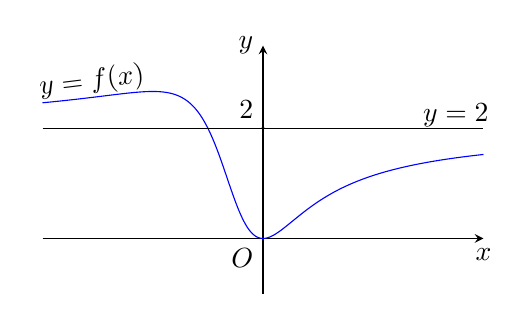
\begin{tikzpicture}[smooth,samples=300,scale=0.7,>=stealth]
\draw[->,>=stealth] (-4,0)--(4,0) node[below]{$x$};
\draw[->,>=stealth] (0,-1)--(0,3.5) node[left]{$y$};
\draw (0,0) node[below left]{$O$};
\draw[blue,	domain=-4:4,samples=400] plot(\x,{2*(\x)^2/((\x)^2 +\x+ 1)});
\draw (-4,2) -- (4,2) node[above,xshift=-10,yshift=-3] {$y = 2$};
\node[rotate=7,yshift =17] at (-3,2) {$y = f(x)$};
\fill (0,2) circle (1pt) node [above left]{$2$};
\end{tikzpicture}
}
\loigiai{
Hàm số đã cho có tập xác định là $\mathbb{R}$. \\
Vì $\lim\limits_{x\to\pm\infty}f(x)=\lim\limits_{x\to\pm\infty}\dfrac{2x^2}{x^2 + x + 1}=2$ nên đường thẳng $y=2$ là một tiệm cận ngang của đồ thị hàm số.
}
\end{ex}
%%%Câu 18%
\begin{ex}%[2D1-Bai3-Dang2-TN]%[Dự án đề cương 3 Khối NH24-25-Dot 1- Bùi Lương Phúc]%[2D1H4-3]
	(\textit{\footnotesize Theo đề thi GKI - THPT Phạm Văn Đồng - Năm học 2024-2025})\\
	Giả sử hàm số $ y=f(x)$ xác định trên $\mathbb{R}\setminus\left\{-1;1\right\}$, liên tục trên mỗi khoảng xác định và có bảng biến thiên như sau:
	\begin{center}
		
\begin{tikzpicture}[>=stealth,scale=1]
			\tikzset{double style/.append style = {draw=\tkzTabDefaultWritingColor,double=\tkzTabDefaultBackgroundColor,double distance=4pt}}
			\tkzTabInit[nocadre=true,lgt=1.5,espcl=2.5,deltacl=0.8]
			{$x$/.7,$f'(x)$ /.7, $f(x)$ /1.5}
			{$-\infty$, $-1$ , $0$ , $1$ , $+\infty$}
			\tkzTabLine{ ,-, d ,-, 0 ,+, d, +, }
			\tkzTabVar {+/$0$,-D+/$-10$ /$10$, -/$8$,  +D-/$10$ /$-\infty$, +/$10$}
		\end{tikzpicture}
	\end{center}
	Gọi số tiệm cận đứng, số tiệm cận ngang, số tiệm cận xiên của đồ thị hàm số $ y=f(x)$ lần lượt là $m$, $n$, $p$. Giá trị của biểu thức $T=2m+3n+p$ bằng 
\choice 
{$4$ }
{\True $8$ }
{$7$ }
{$10$	}	
	\loigiai{
		Hàm số đã cho có tập xác định là $\mathbb{R} \setminus \{-1;1\}$.\\
		$\bullet$ Vì $\lim\limits_{x\to{-1}^-}f(x)=-10$; $\lim\limits_{x\to{-1}^+}f(x)=10$ nên đường thẳng $ x=-1$ không phải là tiệm cận đứng của đồ thị hàm số đã cho.\\
		$\bullet$ Vì $\lim\limits_{x\to1^+}f(x)=-\infty$ nên đường thẳng $ x=1$ là tiệm cận đứng của đồ thị hàm số đã cho.\\
		$\bullet$ Vì $\lim\limits_{x\to+\infty}f(x)=10$ nên đường thẳng $ y=10$ là tiệm cận ngang của đồ thị hàm số đã cho.\\
		$\bullet$ Vì $\lim\limits_{x\to-\infty}f(x)=0$ nên đường thẳng $ y=0$ là tiệm cận ngang của đồ thị hàm số đã cho.\\
		Vậy $m=1$, $n=2$, $p=0$ suy ra $T=2\cdot1+3\cdot2+0=8$.				
	}
\end{ex}
%%%Câu 19%
\begin{ex}%[2D1-Bai3-Dang2-TN]%[Dự án đề cương 3 Khối NH24-25-Dot 1- Bùi Lương Phúc]%[2D1H4-3]
	(\textit{\footnotesize Trích đề thi CKI - THPT Lê Hồng Phong - Năm học 2024-2025})\\
	\immini{Đường cong trong hình vẽ bên là đồ thị của hàm số nào dưới đây?
		\choice[2]
		{$y=\dfrac{x^2+2 x-1}{x-1}$}
		{$y=\dfrac{2 x-1}{x-1}$}
		{\True $y=\dfrac{x+1}{x-1}$}
		{$y=x^3-3 x-1$}
	}{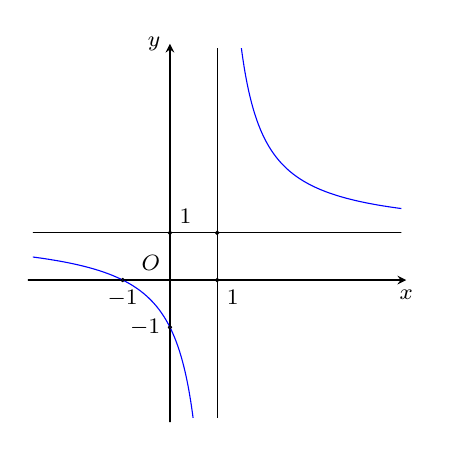
\begin{tikzpicture}[scale=0.6,>=stealth, font=\footnotesize, line join=round, line cap=round]
			\def\a{1} \def\b{1} \def\c{1} \def\d{-1}
			\def\xmin{-3} \def\xmax{5}
			\def\ymin{-3} \def\ymax{5}
			\draw[->] (\xmin,0)--(\xmax,0) node [below]{$x$};
			\draw[->] (0,\ymin)--(0,\ymax) node [left]{$y$};
			\node at (0,0) [above left]{$O$};
			\clip (\xmin+0.1,\ymin+0.1) rectangle (\xmax-0.1,\ymax-0.1);
			\draw[blue,	smooth,samples=200,domain=\xmin:(-\d/\c-0.1)] plot(\x,{(\a*(\x)+\b)/(\c*(\x)+\d)});
			\draw[blue,	smooth,samples=200,domain=(-\d/\c+0.1:\xmax)] plot(\x,{(\a*(\x)+\b)/(\c*(\x)+\d)});
			\draw (-\d/\c,\ymin)--(-\d/\c,\ymax) (\xmin,\a/\c)--(\xmax,\a/\c);
			\draw (1,0) node[below right]{$1$}circle(1pt);
			\draw (0,1) node[above right]{$1$}circle(1pt);
			\draw (-1,0) node[below]{$-1$}circle(1pt);
			\draw (0,-1) node[left]{$-1$}circle(1pt);	
			\draw (1,1) circle(1pt);															
		\end{tikzpicture}
	}	\loigiai{
		Đồ thị hàm số có tiệm cận ngang $y=1$ và tiệm cận đứng $x=1$ nên hàm số cần tìm là $y=\dfrac{x+1}{x-1}$.
	}
\end{ex}
%%%Câu 20%
\begin{ex}%[2D1-Bai3-Dang2-TN]%[Dự án đề cương 3 Khối NH24-25-Dot 1- Bùi Lương Phúc]%[2D1H4-3]
	(\textit{\footnotesize Trích đề thi GKI - THPT Phạm Văn Đồng - Năm học 2024-2025})\\
	\immini{
		Đồ thị đã cho trong hình vẽ là đồ thị hàm số
		\choice[2]
		{$ y=\dfrac{x^2-2x-2}{x+1}$}
		{\True $ y=\dfrac{x^2-2x+2}{x-1}$}
		{$ y=\dfrac{x^2-x+2}{x-1}$}
		{$ y=\dfrac{x^2-2x+3}{x-1}$}
	}{\begin{tikzpicture}[line join=round, line cap=round,>=stealth,scale=0.6]
			\draw[->] (-2.5,0)--(4.5,0) node[below left] {$x$};
			\draw[->] (0,-4)--(0,4) node[below left] {$y$};
			\draw (0,0) node [above left] {$O$};
			\draw (1.01,-4)--(1.01,4);
			\begin{scope}
				%				\clip (-4,-5) rectangle (5,5);
				\draw[blue,	samples=200,domain=-2.5:0.73,smooth,variable=\x] plot (\x,{(1*((\x)^2)-2*(\x)+2)/(1*(\x)-1)});
				\draw[blue,	samples=200,domain=1.27:4.3,smooth,variable=\x] plot (\x,{(1*((\x)^2)-2*(\x)+2)/(1*(\x)-1)});
				\draw(-2.5,-3.6)--(4.3,3.3);
				\draw[dashed] (2,0)--(2,2)--(0,2);
			\end{scope}
			\fill(0,2) circle (1.5pt)($(0,2)+(180:5.5mm)$) node{ $2$} (2,2) circle (1.5pt) (0,-2) circle (1.5pt);
			\fill(2,0) circle (1pt)($(2,0)+(-90:5.0mm)$) node{ $2$};
			\fill(1,0) circle (1pt)($(1,0)+(-45:5.5mm)$) node{ $1$};
			\fill(0,-1) circle (1pt)($(0,-1)+(180:5.5mm)$) node{ $-1$};
			\fill(0,-2) circle (1pt)($(0,-2)+(10:5.5mm)$) node{ $-2$};
	\end{tikzpicture}}
	\loigiai{
		Kiểm tra tọa độ các điểm mà đồ thị đi qua hoặc các đường tiệm cận của đồ thị hàm số, ta loại được các hàm số\\
		$\bullet$ $ y=\dfrac{x^2-x+2}{x-1}=x+\dfrac{2}{x-1}$ (đồ thị hàm số này nhận đường thẳng $ y=x$ làm tiệm cận xiên, không phải đường thẳng $ y=x-1$ như đồ thị đã cho);\\
		$\bullet$ $ y=\dfrac{x^2-2x-2}{x+1}$ (đồ thị hàm số này không nhận đường thẳng $ x=1$ làm tiệm cận đứng);\\
		$\bullet$ $ y=\dfrac{x^2-2x+3}{x-1}$ (đồ thị hàm số này không đi qua điểm (0;-2));\\
		Vậy đồ thị đã cho là đồ thị của hàm số $ y=\dfrac{x^2-2x+2}{x-1}$.}
\end{ex}
\Closesolutionfile{ans}

\ind{PHẦN II.} \inden{Câu trắc nghiệm đúng sai. Trong mỗi ý a), b), c), d) ở mỗi câu, học sinh chọn đúng hoặc sai.}\\
\setcounter{ex}{0}
\Opensolutionfile{ans}[ans/2D1-Bai3-DS]%--Đặt tên 2D1-Bai3-DS
%%CÂU1%
\begin{ex}%[2D1-Bai3-DS]%[Dự án đề cương 3 Khối NH24-25-Dot 1- Bùi Lương Phúc]%[2D1H4-1]
	(\textit{\footnotesize Trích đề thi CKI - THPT Bắc Yên Thành - Năm học 2024-2025})\\
	Cho hàm số $y=\dfrac{x^2+x+2}{x-1}$.
	\choiceTF
	{\True Hàm số có đạo hàm $y'=\dfrac{x^2-2 x-3}{(x-1)^2}$}
	{\True Đồ thị hàm số có đường tiệm cận đứng là $x=1$}
	{Đồ thị hàm số có điểm cực tiểu là $A(-1;-1)$}
	{\True Đường tiệm cận xiên của đồ thị hàm số là $y=x+2$}
	\loigiai{
		Tập xác định $\mathscr{D}=\mathbb{R}\setminus \{1\}$.
		\begin{itemchoice}
			\itemch Ta có $y'=\dfrac{x^2-2x-3}{(x-1)^2}$.
			\itemch Vì $\lim\limits_{x \to 1^+}y=+\infty$ nên đồ thị hàm số có tiệm cận đứng là $x=1$.
			\itemch Cho $y'=0$ ta được $\hoac{ &x=-1 \\ &x=3\\ }$.\\
			Bảng biến thiên của hàm số
			\begin{center}
				
\begin{tikzpicture}
					\tkzTabInit[nocadre=true, lgt=1, espcl=2.5, deltacl=0.5]
					{$x$/0.7,$y'$/0.7,$y$/1.5}
					{$-\infty$,$-1$,$1$,$3$,$+\infty$}
					\tkzTabLine{,+,0,-,d,-,0,+,}
					\tkzTabVar{-/$-\infty$,+/$-1$,-D+/$-\infty$/$+\infty$,-/$7$,+/$+\infty$}
				\end{tikzpicture}
			\end{center}
			Từ bảng biến thiên, suy ra đồ thị hàm số có điểm cực đại $A(-1;-1)$.
			\itemch Ta có $y=x+2+\dfrac{4}{x-1}$ nên đồ thị hàm số có tiệm cận xiên $y=x+2$.
		\end{itemchoice}		
	}
\end{ex}
%%CÂU2%
\begin{ex}%[2D1-Bai3-DS]%[Dự án đề cương 3 Khối NH24-25-Dot 1- Bùi Lương Phúc]%[2D1H4-1]
	(\textit{\footnotesize Trích đề thi GKI - THPT chuyên Nguyễn Quang Diêu - Năm học 2024-2025})\\
	Cho hàm số $y=\dfrac{-x^2-3x+2}{x-3}$ có đồ thị là $(C)$.
	\choiceTF
	{\True Giao điểm giữa $(C)$ và trục tung là điểm $A\left(0;-\dfrac{2}{3}\right)$}
	{\True Đồ thị $(C)$ có tiệm cận đứng là $x=3$}
	{ Đồ thị $(C)$ có tiệm cận xiên là $y=-x+6$}
	{\True Đồ thị $(C)$ có $2$ điểm cực trị nằm về $2$ phía đối với trục $Oy$}
	\loigiai
	{\begin{itemchoice}
			\itemch Sai. Giao điểm giữa $(C)$ và trục tung là điểm $A\left(0;-\dfrac{2}{3}\right)$.
			\itemch Đúng. Ta có $y=-x-6-\dfrac{16}{x-3}$ và $\lim\limits_{x\to 3^-}y=+\infty$, $\lim\limits_{x\to 3^+}y=-\infty$ nên đồ thị $(C)$ có tiệm cận đứng là $x=3$.
			\itemch Đúng. Ta có $y=-x-6-\dfrac{16}{x-3}$ và $\lim\limits_{x\to \pm\infty}\left[y-(-x-6)\right]=\lim\limits_{x\to\pm\infty}\dfrac{-16}{x-3}=0$ nên đồ thị $(C)$ có tiệm cận xiên là $y=-x-6$.\\
			Giao điểm giữa tiệm cận đứng và tiệm cận xiên là điểm $I(3;-9)$.\\
			Vậy đồ thị $(C)$ có tâm đối xứng là điểm $I(3;-9)$.
			\itemch Sai. Ta có $y'=\dfrac{-x^2+6x+7}{(x-3)^2}$ và $y'=0\Leftrightarrow -x^2-6x+7=0\Leftrightarrow\hoac{& x=-1 \\ & x=7.}$\\
			Bảng biến thiên
			\begin{center}
				
\begin{tikzpicture}
					\tkzTabInit[nocadre=false, lgt=1.2, espcl=2.5, deltacl=0.6]
					{$x$/0.6,$y'$/0.6,$y$/1.5}
					{$-\infty$, $-1$, $3$, $7$, $+\infty$}
					\tkzTabLine {,-,0,+,d,+,0,-,}
					\tkzTabVar{+/$+\infty$,-/$-1$, +D-/$+\infty$/$-\infty$, +/$-17$, -/$-\infty$}
				\end{tikzpicture}
			\end{center}
			Đồ thị $(C)$ có các điểm cực trị là $(-1;-1)$ và $(7;-17)$. Các điểm cực trị này cùng nằm phía dưới trục $Ox$.
		\end{itemchoice}
	}
\end{ex}
%%CÂU3%
\begin{ex}%[2D1-Bai3-DS]%[Dự án đề cương 3 Khối NH24-25-Dot 1- Bùi Lương Phúc]%[2D1H4-3]
	(\textit{\footnotesize Trích đề thi CKI - THPT Quế Sơn - Năm học 2024-2025})\\
	Cho hàm số $y = \dfrac{2x-3}{x+1}$ có đồ thị là $(C)$.
	\choiceTF
	{\True Đồ thị $(C)$ của hàm số có tiệm cận ngang là đường thẳng $y = 2$}
	{\True Đồ thị $(C)$ của hàm số có tiệm cận đứng là đường thẳng $x = -1$}
	{\True Đồ thị $(C)$ qua điểm $M(0;-3)$}
	{Tâm đối xứng của $(C)$ nằm trên đường thẳng $\Delta\colon 3x - y + 1 = 0$}
	\loigiai{
		\begin{itemchoice}
			\itemch Tiệm cận ngang là đường thẳng $y = 2$.
			\itemch Tiệm cận đứng là đường thẳng $x = -1$.
			\itemch Vì $-3=\dfrac{2\cdot 0-3}{0+1}$ nên điểm $M(0;-3)$ thuộc $(C)$.
			\itemch Gọi $I$ là tâm đối xứng của $(C)$, khi đó $I(-1;2)$ và $I \not\in \Delta$.
		\end{itemchoice}
	}
\end{ex}
%%CÂU4%
\begin{ex}%[2D1-Bai3-DS]%[Dự án đề cương 3 Khối NH24-25-Dot 1- Bùi Lương Phúc]%[2D1V4-1]
	(\textit{\footnotesize Trích đề thi GKI - THPT Phạm Văn Đồng - Năm học 2024-2025})\\
	Cho hàm số $ y=\dfrac{x+64}{x}$ có đồ thị $(C)$.
	\choiceTF
	{\True $(C)$ có tiệm cận ngang là đường thẳng $ y=1$}
	{\True $(C)$ có tiệm cận đứng là đường thẳng $ x=0$}
	{Hàm số \textbf{không }có giá trị lớn nhất trên tập $\left[2^{-2024};+\infty\right)$}
	{\True Khoảng cách từ một điểm bất kì trên $(C)$ đến tâm đối xứng của $(C)$ có giá trị nhỏ nhất là $ 8\sqrt{2}$}
	\loigiai{
		\begin{itemchoice}
		\itemch Đúng\\
		Vì $\underset{x\to 0^+}{\lim}\,y=\underset{x\to 0^+}{\lim}\,\dfrac{x+64}{x}=+\infty $ nên đường thẳng $ x=0$ là tiệm cận đứng của đồ thị hàm số.
		\itemch Đúng\\
		Vì $\underset{x\to+\infty}{\lim}\,y=\underset{x\to+\infty}{\lim}\,\dfrac{x+64}{x}=\underset{x\to+\infty}{\lim}\,\left(1+\dfrac{64}{x}\right)=1$ nên đường thẳng $ y=1$ là tiệm cận ngang của đồ thị hàm số.
		\itemch Sai.\\
		Vì $y'=-\dfrac{64}{x^2}<0,\forall x\ne 0$ nên hàm số nghịch biến trên $\left[2^{-2024};+\infty\right)$. Suy ra giá trị lớn nhất của hàm số trên $\left[2^{-2024};+\infty\right)$ là $f\left(2^{-2024}\right)=1+2^{2030}$.\\
		Vậy hàm số đã cho có giá trị lớn nhất trên $\left[2^{-2024};+\infty\right)$ và giá trị đó là $f\left(2^{-2024}\right)=1+2^{2030}$.
		\itemch 
		Đồ thị $(C)$ có tâm đối xứng là giao điểm của hai đường tiệm cận, đó là $ I\left(0;1\right)$.\\
		Lấy $ M\left(x;1+\dfrac{64}{x}\right)$ thuộc $(C)$, ta có\\
		$IM=\sqrt{\left(x-0\right)^2+\left(1+\dfrac{64}{x}-1\right)^2}=\sqrt{x^2+\left(\dfrac{64}{x}\right)^2}$\\
		$=\sqrt{\left(x-\dfrac{64}{x}\right)^2+128}\ge\sqrt{128}=8\sqrt{2}$.\\
		Đẳng thức xảy ra khi $ x-\dfrac{64}{x}=0\Leftrightarrow x=\pm 8$.
		\end{itemchoice}
		}
\end{ex}
%%CÂU5%
\begin{ex}%[2D1-Bai3-DS]%[Dự án đề cương 3 Khối NH24-25-Dot 1- Bùi Lương Phúc]%[2D1H4-4]
	Nồng độ oxygen trong hồ theo thời gian $t$ là một hàm số cho bởi công thức $y=5-\dfrac{15t}{9t^2+1}$, với $y$ được tính theo mg/l và $t$ được tính theo giờ, $t\ge 0$.
	\choiceTF
	{Đồ thị hàm số $y=5-\dfrac{15t}{9t^2+1}$ có một đường tiệm cận ngang và một đường tiệm cận xiên}
	{\True Đồ thị hàm số có đường tiệm cận ngang là $y=5$}
	{Đồ thị hàm số có đường tiệm cận đứng là $x=\dfrac{1}{3}$}
	{\True Sau một thời gian đủ dài, nồng độ oxygen trong hồ sẽ bão hòa và đạt ngưỡng $5$\,mg/l.}
	\loigiai{
		\begin{itemchoice}
			\itemch $\lim\limits_{t\to+\infty}y=\lim\limits_{t\to+\infty}\left(5-\dfrac{\dfrac{15}{t}}{9+\dfrac{1}{t^2}}\right)=5$. Vậy đồ thị hàm số không có đường tiệm cận xiên.
			\itemch $\lim\limits_{t\to+\infty}y=\lim\limits_{t\to+\infty}\left(5-\dfrac{\dfrac{15}{t}}{9+\dfrac{1}{t^2}}\right)=5$. Vậy đồ thị hàm số có đường tiệm cận ngang là $y=5$.
			\itemch Do $9t^2+1>0\ \forall t\in\mathbb{R}$ nên tập xác định của hàm số là $\mathbb{R}$. Vậy đồ thị hàm số không có đường tiệm cận đứng.
			\itemch $\lim\limits_{t\to+\infty}y=5$ nên sau một thời gian đủ dài, nồng độ oxygen trong hồ sẽ bão hòa và đạt ngưỡng $5$\,mg/l.
		\end{itemchoice}		
	}
\end{ex}

\Closesolutionfile{ans}

\ind{PHẦN III.} \inden{Câu trắc nghiệm trả lời ngắn. Trong mỗi câu, học sinh điền kết quả.}\\
\setcounter{ex}{0}
\Opensolutionfile{ans}[ans/2D1-Bai3-TLN]%--Đặt tên 2D1-Bai3-TLN
%%%Cau1%
\begin{ex}%[2D1-Bai3-TLN]%[Dự án đề cương 3 Khối NH24-25-Dot 1- Bùi Lương Phúc]%[2D1V4-1]
Cho hàm số $y = \dfrac{2x}{x^2 - 4}$. Gọi số tiệm cận đứng và số tiệm cận ngang của đồ thị hàm số lần lượt là $m$, $n$. Giá trị biểu thức $T=3m+2n$ bằng bao nhiêu?
\shortans{$8$}
\loigiai{
Hàm số đã cho có tập xác định là $\mathbb{R} \setminus \{-2;2\}$. \\
Vì $\lim\limits_{x\to-2^-}y=-\infty$, $\lim\limits_{x\to-2^+}y=+\infty$ nên đồ thị hàm số có tiệm cận đứng là đường thẳng $x = -2$.\\
Vì $\lim\limits_{x\to2^-}y=+\infty$, $\lim\limits_{x\to2^+}y=-\infty$ nên đồ thị hàm số có tiệm cận đứng là đường thẳng $x = 2$.\\
Vì $\lim\limits_{x\to\pm\infty}y=0$ nên đồ thị hàm số có tiệm cận ngang là đường thẳng $y = 0$.\\
Vậy $m=2$, $n=1$ suy ra $T=3\cdot2+2\cdot1=8$.
}
\end{ex}
%%%Cau2%
\begin{ex}%[2D1-Bai3-TLN]%[Dự án đề cương 3 Khối NH24-25-Dot 1- Bùi Lương Phúc]%[2D1V4-1]
	(\textit{\footnotesize Trích đề thi GKI - THPT chuyên Nguyễn Quang Diêu - Năm học 2024-2025})\\
	\immini{Cho hàm số $y=\dfrac{ax+2}{cx+d}$ có đồ thị $(C)$ như hình vẽ bên dưới. Giá trị biểu thức $T=a^2+c^2+d^2$ bằng bao nhiêu?}{
		\begin{tikzpicture}[line join=round, line cap=round,>=stealth,scale=0.5]
			\def\a{1}
			\def\b{2}
			\def\c{1}
			\def\d{-2}
			\def\f(#1){(\a*(#1)+\b)/(\c*(#1)+\d)}
			\def\xmin{-3}
			\def\xmax{7}
			\def\ymin{-4}
			\def\ymax{6}
			\def\m{-\d/\c}
			\def\n{0.8}
			\draw[->] (\xmin,0)--(\xmax,0) node[below] { $x$};
			\draw[->] (0,\ymin)--(0,\ymax) node[left] { $y$};
			\draw (0,0)  circle (1pt) node [below right] { $O$};
			\draw (-\d/\c,\ymin)--(-\d/\c,\ymax) (\xmin,\a/\c)--(\xmax,\a/\c);
			\draw[blue,smooth,samples=200] plot[domain=\xmin:{\m-\n}] (\x,{\f(\x)});
			\draw[blue,smooth,samples=200] plot[domain={\m+\n}:\xmax] (\x,{\f(\x)});
			\fill (-2,0) circle (1pt) node[below]{$-2$}
			(0,-1) circle (1pt) node[left]{$-1$}
			(2,0) circle (1pt) node[below right]{$2$}
			(0,1) circle (1pt) node[above left]{$1$};
		\end{tikzpicture}
	}
		\shortans{$6$}
		\loigiai{
		Dựa vào đồ thị hàm số $(C)$ ta có
		Đường tiệm cận đứng $x=-\dfrac{d}{c}=2\Rightarrow d=-2c$\quad $(1)$.\\
		Đường tiệm cận ngang $y=\dfrac{a}{c}=1\Rightarrow a=c$\quad $(2)$.\\
		$(C)$ đi qua điểm $A(0;-1)$ nên $\dfrac{2}{d}=-1\Rightarrow d= -2$\quad $(3)$.\\
		Từ $(1)$, $(2)$, $(3)$ suy ra $d=-2$, $c=a=1$.\\
		Vậy $T=1^2+1^2+(-2)^2=6$.
	}
\end{ex}
%%Cau3%
\begin{ex}%[2D1-Bai3-TLN]%[Dự án đề cương 3 Khối NH24-25-Dot 1- Bùi Lương Phúc]%[2D1V4-1]
Cho hàm số bậc ba $f(x)=x^3+ax^2+bx+c$. Biết rằng đồ thị hàm số cắt trục hoành tại $3$ điểm phân biệt đều có hoành độ dương. Đồ thị hàm số $y =g(x)= \dfrac{x+1}{f(x)}$ có bao nhiêu tiệm cận?
\shortans{$4$}
\loigiai{
Từ giả thiết suy ra, đồ thị hàm số $f(x)=x^3+ax^2+bx+c$ cắt trục hoành tại $3$ điểm phân biệt có hoành độ dương là $x_1$, $x_2$, $x_3$, tức là $0<x_1<x_2<x_3$. Khi đó $f(x)=(x-x_1)(x-x_2)(x-x_3)$.\\
Xét hàm số $y =f(x) =(x-x_1)(x-x_2)(x-x_3)$.\\
\begin{center}
\begin{tikzpicture}
\tkzTabInit[nocadre=true, lgt=1, espcl=2.5, deltacl=0.5]
{$x$/0.7,$y$/1.5}
{$-\infty$,$ $,$ $,$+\infty$}
\tkzTabVar{-/$ $,+/$ $,-/$ $,+/$ $}
\tkzTabVal[draw]{1}{2}{0.5}{$x_1$}{$0$}
\tkzTabVal[draw]{2}{3}{0.5}{$x_2$}{$0$}
\tkzTabVal[draw]{4}{3}{0.5}{$x_3$}{$0$}
\draw[blue](1.5,-1.5)--(9,-1.5) node [above]{$Ox$};
\end{tikzpicture}
\end{center}
Hàm số $g(x)=\dfrac{x+1}{(x-x_1)(x-x_2)(x-x_3)}$ có tập xác định là $\mathbb{R} \setminus \{x_1; x_2; x_3\}$. \\
Vì $\lim\limits_{x\to {x_1}^-}g(x)=-\infty$, $\lim\limits_{x\to{x_1}^+}y=+\infty$ nên đồ thị hàm số có tiệm cận đứng là đường thẳng $x = x_1$.\\
Vì $\lim\limits_{x\to {x_2}^-}g(x)=+\infty$, $\lim\limits_{x\to{x_2}^+}y=-\infty$ nên đồ thị hàm số có tiệm cận đứng là đường thẳng $x = x_2$.\\
Vì $\lim\limits_{x\to {x_3}^-}g(x)=-\infty$, $\lim\limits_{x\to{x_3}^+}y=+\infty$ nên đồ thị hàm số có tiệm cận đứng là đường thẳng $x = x_3$.\\
Vì $\lim\limits_{x\to\pm\infty}g(x)=\lim\limits_{x\to\pm\infty}\dfrac{\dfrac{1}{x^2}+\dfrac{1}{x^3}}{\left(1-\dfrac{x_1}{x}\right) \left(1-\dfrac{x_2}{x}\right) \left(1-\dfrac{x_2}{x}\right)}=0$ nên đồ thị hàm số có tiệm cận ngang là đường thẳng $y = 0$.\\
Vậy đồ thị hàm số đã cho có $4$ tiệm cận (là các đường thẳng $x = x_1$, $x = x_2$, $x = x_3$ và $y = 0$).
}
\end{ex}
%%%Cau4%
\begin{ex}%[du_an_Qrcode_vo_tu_hoc_Bui-Luong-Phuc]%[2D1V4-1]
	Cho hàm số $y=f(x)=\dfrac{x+2}{x-3}$ có đồ thị $(C)$. Gọi tổng khoảng cách từ mỗi điểm $M(x,y)\in(C)$, với $x>3$, tới hai đường tiệm cận của $(C)$ là $g(x)$. Góc giữa đường tiệm cận xiên của đồ thị hàm số $y=g(x)$ và trục hoành bằng bao nhiêu độ?
	\shortans{$45$}
	\loigiai{
		Hàm số đã cho có tập xác định là $\mathbb{R} \setminus \{3\}$. \\
		Vì $\lim\limits_{x\to3^+}f(x)=+\infty$ nên đồ thị hàm số $y=f(x)$ có tiệm cận đứng là đường thẳng $x = 3$.\\
		Vì $\lim\limits_{x\to+\infty}f(x)=1$ nên đồ thị hàm số $y=f(x)$ có tiệm cận ngang là đường thẳng $y = 1$.\\
		Khoảng cách từ mỗi điểm $M(x,y)\in(C)$, với $x>3$, tới đường thẳng $x = 3$ là $x-3$.\\
		Khoảng cách từ mỗi điểm $M(x,y)\in(C)$, với $x>3$, tới đường thẳng $y = 1$ là $y-1=\dfrac{x+2}{x-3}-1=\dfrac{5}{x-3}$.\\
		Tổng khoảng cách từ mỗi điểm $M(x,y)\in(C)$ (với $x>3$) tới hai đường tiệm cận của $(C)$ là $g(x)=x-3+\dfrac{5}{x-3}$.\\
		Ta có
		$\lim\limits_{x\to3^+}g(x)=+\infty$ nên đồ thị hàm số $y=g(x)$ có tiệm cận đứng là đường thẳng $x = 3$.\\
		$\lim\limits_{x\to+\infty}\left[g(x)-(x-3)\right]=\dfrac{5}{x-3}=0$ nên đồ thị hàm số $y=g(x)$ có tiệm cận xiên là đường thẳng $y = x-3$.\\
		Đường thẳng $y = x-3$ có hệ số góc bằng $1$.\\
		Gọi $\alpha$ là góc giữa tiệm cận xiên và trục hoành thì $\tan \alpha=1\Rightarrow \alpha=45^\circ$.
	}
\end{ex}
%%Cau5%
\begin{ex}%[2D1-Bai3-TLN]%[Dự án đề cương 3 Khối NH24-25-Dot 1- Bùi Lương Phúc]%[2D1V4-4]
	(\textit{\footnotesize Theo SGK Cánh Diều 12})\\
Có một bình có dung tích $5\,000$\,ml. Trong bình có chứa $200$\,ml dung dịch muối với nồng độ $5$\,mg/ml. Cần thêm tối thiểu bao nhiêu mililit dung dịch muối với nồng độ $10$\,mg/ml vào bình để có dung dịch muối với nồng độ lớn hơn $9{,}8$\,mg/ml?
\shortans{$4\,801$}
\loigiai{	
	Số gam muối tinh chất có trong bình lúc đầu là $5\cdot200=1\,000$\,mg.\\
	Gọi $x$\,ml dung dịch muối với nồng độ $10$\,mg/ml được thêm vào bình. Khi đó lượng muối tinh chất thêm vào là $10x$\,mg.\\
	Tổng lượng muối tinh chất sau khi thêm $x$\,ml vào bình là $1\,000+10x$.\\
	Nồng độ muối mới là $f(x)=\dfrac{1\,000+10x}{200+x}$.\\
	Giải điều kiện $f(x)>9{,}8\Leftrightarrow\dfrac{1\,000+10x}{200+x}>9{,}8\Leftrightarrow x>4\,800$.\\
Vậy phải đổ thêm vào bình tối thiểu là $4\,801$\,ml.
	}
\end{ex}	
\Closesolutionfile{ans}

\ind{PHẦN IV.} \inden{Tự luận.}\\
\setcounter{ex}{0}
\Opensolutionfile{ans}[ans/2D1-Bai3-TL]%--Đặt tên 2D1-Bai3-TL
%%%Câu 1%
\begin{ex}%[2D1-Bai3-TL]%[Dự án đề cương 3 Khối NH24-25-Dot 1- Bùi Lương Phúc]%[2D1N4-1]
Cho hàm số $y = f(x)$ có bảng biến thiên như sau:
\begin{center}

\begin{tikzpicture}
\tkzTabInit[nocadre=true, lgt=1, espcl=4, deltacl=0.5]
{$x$/0.7,$y’$/0.7,$y$/1.5}
{$-\infty$,$2$,$+\infty$}
\tkzTabLine{,+,d,+,}
\tkzTabVar{-/$-2$,+D-/$+\infty$/$-\infty$,+/$-2$}
\end{tikzpicture}
\end{center}
Chỉ ra phương trình các đường tiệm cận của đồ thị hàm số đã cho. Giải thích?\\
\dapso{$x=2$, $y=-2$.}
\loigiai{
Hàm số đã cho có tập xác định là $\mathbb{R} \setminus \{2\}$. \\
Đồ thị hàm số đã cho có $1$ tiệm cận đứng $x=2$ và  $1$ tiệm cận ngang $y=-2$ vì\\
$\lim\limits_{x\to2^+}y=-\infty$, $\lim\limits_{x\to2^-}y=+\infty$ nên đường thẳng $x=2$ là một tiệm cận đứng của đồ thị hàm số. \\
$\lim\limits_{x\to\pm\infty}y=-2$ nên đường thẳng $y=-2$ là một tiệm cận ngang của đồ thị hàm số.
}
\end{ex}
%%%Câu 2%
\begin{ex}%[2D1-Bai3-TL]%[Dự án đề cương 3 Khối NH24-25-Dot 1- Bùi Lương Phúc]%[2D1N4-1]
	(\textit{\footnotesize Theo đề thi CKI - THPT Quế Sơn - Năm học 2024-2025})\\
	Tìm phương trình đường tiệm cận xiên của đồ thị hàm số $y =x-\dfrac{4}{x-1}$.\\
	\dapso{$x=1$, $y=x$.}
	\loigiai{
		Vì $\lim\limits_{x\to\pm\infty}\left[f(x)-x\right]=\lim\limits_{x\to\pm\infty}\dfrac{-4}{x-1}=0$ nên đường thẳng $y=x$ là tiệm cận xiên của đồ thị hàm số đã cho.
	}
\end{ex}
%%%Câu 3%
\begin{ex}%[2D1-Bai3-TL]%[Dự án đề cương 3 Khối NH24-25-Dot 1- Bùi Lương Phúc]%[2D1H4-1]
Cho hàm số $y = -x + 3 - \dfrac{5}{2x + 1}$ có đồ thị $(C)$. Tính khoảng cách từ gốc tọa độ $O$ đến giao điểm của hai tiệm cận của $(C)$.\\
\dapso{$\dfrac{5\sqrt{2}}{2}$.}
\loigiai{
Hàm số đã cho có tập xác định là $\mathbb{R} \setminus \left\{-\dfrac{1}{2}\right\}$. \\
Vì $\lim\limits_{x\to{\tfrac{-1}{2}}^-}y=+\infty$, $\lim\limits_{x\to{\tfrac{-1}{2}}^+}y=-\infty$ nên đường thẳng $x=-\dfrac{1}{2}$ là một tiệm cận đứng của đồ thị hàm số. \\
Vì $\lim\limits_{x\to\pm\infty}\left[y-(-x+3)\right]= \lim\limits_{x \to \pm\infty} \dfrac{-5}{2x+1} = 0$ nên đường thẳng $y=-x+3$ là một tiệm cận xiên của đồ thị hàm số.\\
Gọi giao điểm của hai tiệm cận của $(C)$ là $I$. Tọa độ điểm $I$ thỏa mãn hệ phương trình
\[\left\{\begin{array}{l}x = -\dfrac{1}{2} \\y = -x+3	\end{array}	\right.
\Leftrightarrow
\left\{\begin{array}{l}	x = -\dfrac{1}{2} \\y = \dfrac{7}{2}	\end{array}	\right.
\Rightarrow I\left(-\dfrac{1}{2};\dfrac{7}{2}\right).\]
Vậy $OI=\sqrt{\left(-\dfrac{1}{2}\right)^2+\left(\dfrac{7}{2}\right)^2}=\dfrac{5\sqrt{2}}{2}$.
}
\end{ex}	
%%%Câu 4%
\begin{ex}%[2D1-Bai3-TL]%[Dự án đề cương 3 Khối NH24-25-Dot 1- Bùi Lương Phúc]%[2D1H4-1]
Cho hàm số $y = \dfrac{4}{2 - x}$ có đồ thị $(C)$. Gọi $M$ là điểm nằm trên $(C)$, có hoành độ lớn hơn $2$ và cách đều hai đường tiệm cận của $(C)$. Tìm tung độ của điểm $M$.\\
\dapso{$x=2$, $y=0$.}
\loigiai{
Hàm số đã cho có tập xác định là $\mathbb{R} \setminus \{2\}$. \\
Vì $\lim\limits_{x\to2^+}y=+\infty$, $\lim\limits_{x\to2^-}y=-\infty$ nên đồ thị hàm số có tiệm cận đứng là đường thẳng $d\colon x=2$.\\
Vì $\lim\limits_{x\to\pm\infty}y=0$ nên đồ thị hàm số có tiệm cận ngang là đường thẳng $y=0$, là trục $Ox$.\\
Gọi $M(x_0;y_0)\in(C)$ với $x_0>2$. Ta có $y_0=\dfrac{4}{2-x_0}$.\\
$\bullet\ \mathrm{d}(M,d)=|x_0-2|=x_0-2$; \\
$\bullet\ \mathrm{d}(M,Ox)=|y_0|=\left|\dfrac{4}{2-x_0}\right|=\dfrac{4}{x_0-2}$.\\
Theo bài ra, $\mathrm{d}(M,d)=\mathrm{d}(M,Ox)\Leftrightarrow x_0-2=\dfrac{4}{x_0-2}\Leftrightarrow (x_0-2)^2=4\Leftrightarrow x_0=4$ (vì $x_0>2$).\\
Vậy $y_0=\dfrac{4}{2-4}=-2$.
}
\end{ex}
%%%Câu 5%
\begin{ex}%[2D1-Bai3-TL]%[Dự án đề cương 3 Khối NH24-25-Dot 1- Bùi Lương Phúc]%[2D1H4-1]
	(\textit{\footnotesize Theo SGK Cánh Diều 12})\\
Cho hàm số $y=f(x)=\dfrac{\sqrt{x^2+3}}{x-1}$. Hãy tìm các tiệm cận đứng và tiệm cận ngang của đồ thị hàm số đã cho.\\
	\dapso{$4$.}
\loigiai{ 
	Hàm số đã cho có tập xác định là $\mathbb{R} \setminus \{-1\}$. \\	
	Ta có 
	$\lim\limits_{x \to + \infty} y=\lim\limits_{x \to + \infty } \dfrac{\sqrt{1+\dfrac{3}{x^2}}}{1-\dfrac{1}{x}}=1$; 
	$\lim\limits_{x \to - \infty} y=\lim\limits_{x \to - \infty } \dfrac{-\sqrt{1+\dfrac{3}{x^2}}}{1-\dfrac{1}{x}}=-1$;
	$\lim\limits_{x \to 1^-} y=- \infty$;
	$\lim\limits_{x \to 1^+} y=+ \infty$.\\
	Suy ra đồ thị hàm số có $2$ tiệm cận ngang là $y=\pm1$ và $2$ tiệm cận đứng là $x=\pm1$.
}
\end{ex}
%%%Câu 6%
\begin{ex}%[2D1-Bai3-TL]%[Dự án đề cương 3 Khối NH24-25-Dot 1- Bùi Lương Phúc]%[2D1H4-1]
	(\textit{\footnotesize Theo đề thi GKI - THPT chuyên Nguyễn Quang Diêu - Năm học 2024-2025})\\
	Tìm đường tiệm cận xiên của đồ thị hàm số $y=\dfrac{12 x^2 + 3 x - 14}{3 - 4 x}$ cắt hai trục tọa tọa độ lần lượt tại $A$ và $B$. Tính diện tích tam giác $OAB$.\\
	\dapso{$\dfrac{3}{2}$.}
	\loigiai{ 
	Viết lại $y=\dfrac{12 x^{2} + 3 x - 14}{3 - 4 x}=- 3 x - 3 - \dfrac{5}{3 - 4 x}$.\\	
	$\lim\limits_{x \to \pm \infty} \left[y -(- 3 x - 3)\right]=\lim\limits_{x \to \pm \infty } \dfrac{-5}{3 - 4 x}=0$.\\
	Đường tiệm cận xiên $d$ của đồ thị hàm số là $y=- 3 x - 3$. 
	Ta có $d\cap Oy=A(0;-3)\Rightarrow OA=3$, $d\cap Ox=B(-1;0)\Rightarrow OB=1$.\\
	Tam giác $OAB$ vuông tại $O$ nên diện tích tam giác $OAB$ là\\
	\[S_{OAB}=\dfrac{1}{2}\cdot OA\cdot OB=\dfrac{1}{2}\cdot 3\cdot 1=\dfrac{3}{2}.\] 
	}
\end{ex}
%%%Cau7%
\begin{ex}%[2D1-Bai3-TL]%[Dự án đề cương 3 Khối NH24-25-Dot 1- Bùi Lương Phúc]%[2D1H4-1]
	(\textit{\footnotesize Trích đề thi GKI - THPT chuyên Nguyễn Quang Diêu - Năm học 2024-2025})
	\immini{Đồ thị $(C)$ của hàm số $y=\dfrac{ax^2+bx+c}{x+1}$ là đường cong như hình vẽ bên. Tìm hệ số góc của đường tiệm cận xiên của đồ thị hàm số đã cho}{
		\begin{tikzpicture}[scale=1, font=\footnotesize, line join=round, line cap=round,>=stealth,x=0.4cm,y=0.4cm]
			\def \xmin{-7};
			\def \xmax{5};
			\def \ymin{-7.5};
			\def \ymax{6.5};
			\draw[->] (\xmin, 0.) -- (\xmax,0.) node[anchor=north] {$x$};
			\draw[->] (0.,\ymin) -- (0.,\ymax) node[anchor=west] {$y$};
			\clip(\xmin+0.1,\ymin+0.1) rectangle (\xmax-0.1,\ymax-0.1);
			\draw[blue,smooth,samples=300,domain=\xmin:-1.01] plot(\x,{(-(\x)^2-3*(\x)-6)/((\x)+1)});
			\draw[blue,smooth,samples=300,domain=-0.99:\xmax] plot(\x,{(-(\x)^2-3*(\x)-6)/((\x)+1)});
			%			\draw[smooth,samples=200,domain=\xmin:\xmax] plot(\x,{-(\x)-2});
			\draw (-1,\ymin)--(-1,\ymax);
			\draw[dashed] (-3,0)node[below]{$-3$}|-(0,3)node[right]{$3$} (1,0)node[above]{$1$}|-(0,-5);
			\foreach \x/\y/\l/\g in {0/0/O/-135,0/3//0,1/0//0,-1/0/-1/-135,-3/0//0,0/-5/-5/170,-3/3//0,1/-5//0,0/-6/-6/170}{\fill (\x,\y) circle(1pt)+(\g:0.6) node{$\l$};}
		\end{tikzpicture}
	}
	\dapso{$-1$}
	\loigiai
	{Viết lại $y=f(x)=\dfrac{ax^2 + bx +c}{x+1}=ax +b-a+ \dfrac{a-b+c}{x+1}$.\\
	Ta có $f'(x)=a- \dfrac{a-b+c}{(x+1)^2}$.\\
	Vì $(C)$ có hai điểm cực trị là $(-3;3)$ và $(1;-5)$ nên 
	\[\left\{\begin{array}{l}
		f(-3)=3 \\f(1)=-5 \\f'(1)=0
	\end{array}\right.
	\Leftrightarrow
	\left\{\begin{array}{l} \dfrac{9a -3b +c}{-2}=3 \\ \dfrac{a + b +c}{2}=-5 \\ a-\dfrac{a- b+c}{4}=0 \end{array}\right.
	\Leftrightarrow
	\left\{\begin{array}{l} 9a -3b +c=-6 \\ a + b +c=-10 \\ 3a+ b-c=0 \end{array}\right.
	\Leftrightarrow
	\left\{\begin{array}{l} a =-1 \\ b =-3 \\ c=-6. \end{array}\right.	
	\]
	Vậy $y=f(x)=\dfrac{-x^2 -3x -6}{x+1}=-x -2- \dfrac{4}{x+1}$.\\
	Vì $\lim\limits_{x \to \pm \infty} \left[y -(- x - 2)\right]=\lim\limits_{x \to \pm \infty } \dfrac{-4}{x+1}=0$ nên đồ thị hàm số có tiệm cận xiên $d$ là $y=-x-2$ .\\
	Vậy $d$ có hệ số góc là $-1$. 
	}
\end{ex}
%%%Cau8%
\begin{ex}%[2D1-Bai3-TL]%[Dự án đề cương 3 Khối NH24-25-Dot 1- Bùi Lương Phúc]%[2D1V4-4]
Tốc độ đánh máy trung bình $S$ (tính bằng từ/phút) của một học viên sau $t$ tuần học được cho bởi công thức $S(t) = \dfrac{100t^2}{65 + t^2}$.
\begin{itemize}
\item[a)] Xem $y = S(t) = \dfrac{100t^2}{65 + t^2}$ là một hàm số xác định trên khoảng $(0; +\infty)$, hãy tìm tiệm cận ngang của đồ thị hàm số đó.
\item[b)] Nêu nhận xét về tốc độ đánh máy trung bình của học viên đó khi thời gian $t$ càng lớn.
\end{itemize}
\dapso{$100$.}
\loigiai{
\begin{itemize}
\item[a)] Ta có $\lim\limits_{t\to +\infty}S(t)=\lim\limits_{t\to +\infty}\dfrac{100t^2}{65 + t^2}=\lim\limits_{t\to +\infty}\dfrac{100}{\dfrac{65}{t^2}+1}=100$. \\
Suy ra tiệm cận ngang của đồ thị hàm số là đường thẳng $y=100$.
\item[b)] Khi thời gian $t$ ngày càng lớn, tốc độ đánh máy trung bình của học viên tuy thay đổi nhưng chỉ dần đạt ngưỡng $100$\,từ/phút.
\end{itemize}
}
\end{ex}
%%%Cau9%
\begin{ex}%[2D1-Bai3-TL]%[Dự án đề cương 3 Khối NH24-25-Dot 1- Bùi Lương Phúc]%[2D1V4-4]
Tổng chi phí để sản xuất $x$ sản phẩm của một xí nghiệp được tính theo công thức
$T(x) = 20x + 100\,000$ (đơn vị: nghìn đồng).
\begin{itemize}
\item[a)] Viết công thức tính chi phí trung bình $C(x)$ của $1$ sản phẩm khi sản xuất được $x$ sản phẩm.
\item[b)] Xem $y = C(x)$ là một hàm số xác định trên khoảng $(0; +\infty)$, hãy lập bảng biến thiên của hàm số đó.
\item[c)] Nêu nhận xét về chi phí để tạo ra $1$ sản phẩm khi $x$ càng lớn.
\end{itemize}
\dapso{$20$.}
\loigiai{
\begin{itemize}
\item[a)] $C(x)=20 + \dfrac{100\,000}{x}$ (nghìn đồng/sản phẩm).
\item[b)] Xét hàm số $y = C(x)=20 + \dfrac{100\,000}{x}$ trên khoảng $(0; +\infty)$.\\
$C'(x)=-\dfrac{100\,000}{x^2}<0\ \forall x>0$ nên hàm số nghịch biến trên khoảng $(0; +\infty)$;\\
$\lim\limits_{t\to 0^+}C(t)=+\infty$ nên đồ thị hàm số có tiệm cận đứng $x=0$;\\	$\lim\limits_{t\to +\infty}C(t)=20$ nên đồ thị hàm số có tiệm cận ngang $y=20$;\\
Ta có bảng biến thiên như sau:
\begin{center}
\begin{tikzpicture}
\tkzTabInit[nocadre=true, lgt=1, espcl=4, deltacl=0.5]
{$x$/0.7,$y’$/0.7,$y$/1.5}
{$0$,$+\infty$}
\tkzTabLine{d,-,}
\tkzTabVar{D+/$+\infty$,-/$20$}
\fill[pattern = north west lines,opacity=0.3] (1,-2.9)rectangle (1.5,-0.7);
\end{tikzpicture}
\end{center}
\item[c)] Khi số sản phẩm được tạo ra càng lớn, chi phí càng giảm dần về ngưỡng $20$\,nghìn đồng/sản phẩm.
\end{itemize}
}
\end{ex}
%%%Cau10%
\begin{ex}%[2D1-Bai3-TL]%[Dự án đề cương 3 Khối NH24-25-Dot 1- Bùi Lương Phúc]%[2D1C4-4]
	(\textit{\footnotesize Trích đề thi CKI - THPT Số 1 Văn Bàn - Năm học 2024-2025})\\
	Một bể chứa $8\,000$ lít nước tinh khiết. Người ta bơm vào bể đó nước muối có nồng độ $50$ gam muối cho mỗi lít nước với tốc độ $25$ lít/phút.
	\begin{itemize}
	\item[a)] Tìm hàm số biểu thị nồng độ muối trong bể sau $t$ phút.
	\item[b)] Nêu nhận xét về nồng độ muối trong bể sau thời gian $t$ ngày càng lớn.
	\end{itemize}
	\dapso{$50$.}	
	\loigiai{
	\begin{itemize}
	\item[a)] Sau $t$ phút số lượng muối trong bể là $25t\cdot50=1\,250t$ (gam).\\
			Lượng nước trong bể lúc này là $25t+8\,000$ (lít).\\
			Nồng độ muối trong bể sau $t$ phút là 
			$f(t)=\dfrac{1\,250t}{25t+8\,000}$ (gam/lít).\\
			Vậy hàm số biểu thị nồng độ muối trong bể sau $t$ phút là $f(t)=\dfrac{1\,250t}{25t+8\,000}$ (gam/lít). 
	\item[b)] Khi thời gian $t$ càng lớn thì ta có
			\[\lim\limits_{t\to +\infty}f(t)=\lim\limits_{t\to +\infty}\dfrac{1\,250t}{25t+8\,000}=\lim\limits_{t\to +\infty}\dfrac{1\,250}{25+\dfrac{8\,000}{t}}=\dfrac{1\,250}{25}=50.\]
			Vậy khi thời gian $t$ ngày càng lớn thì nồng độ muối trong bể cũng tăng dần đến $50$\, gam/lít.
		\end{itemize}
	}
\end{ex}
\Closesolutionfile{ans}




